\documentclass[11pt]{article}
\usepackage[T1]{fontenc}
\usepackage{lmodern,microtype}
\usepackage[a4paper,margin=26mm]{geometry}
\usepackage{amsmath,amssymb,amsthm,mathtools}
\usepackage{graphicx,booktabs,array}
\usepackage[dvipsnames]{xcolor}
\usepackage[colorlinks=true,linkcolor=MidnightBlue,citecolor=MidnightBlue,urlcolor=MidnightBlue]{hyperref}
\usepackage{enumitem,fancyhdr}
\setlist{nosep}
\setlength{\emergencystretch}{2em}
\newtheorem{theorem}{Theorem}[section]
\newtheorem{lemma}[theorem]{Lemma}
\newtheorem{corollary}[theorem]{Corollary}
\newtheorem{proposition}[theorem]{Proposition}
\theoremstyle{remark}\newtheorem{remark}[theorem]{Remark}
\newcommand{\eps}{\varepsilon}
\newcommand{\C}{\mathcal C}
\newcommand{\Hcal}{\mathcal H}
\newcommand{\sgn}{\operatorname{sgn}}
\newcommand{\asinh}{\operatorname{arsinh}}
\newcommand{\atanh}{\operatorname{artanh}}
\newcommand{\Real}{\operatorname{Re}}
\newcommand{\Imag}{\operatorname{Im}}
\newcommand{\norm}[1]{\left\lVert#1\right\rVert}
\pagestyle{fancy}\fancyhf{}
\fancyhead[L]{\small Moment-calibrated Wiener--Hopf factors}
\fancyhead[R]{\small S. Gupta}
\fancyfoot[C]{\thepage}
\setlength{\headheight}{14pt}
\title{\bfseries Sharp Phase Budgets for\\Moment-Calibrated Scalar Wiener--Hopf Factors}
\author{Shivam Gupta\\
\small Independent Researcher, India\\
\small\href{mailto:shivam1720406@gmail.com}{shivam1720406@gmail.com}}
\date{17 October 2026}
\begin{document}
\maketitle
\begin{abstract}
A positive scalar kernel can be accurately known in magnitude while its normalized
Wiener--Hopf factor remains sensitive in phase. We quantify how much a finite set
of calibrated logarithmic moments resolves this ambiguity. For real log-kernel
errors supported on a band, bounded by $\eps$, and annihilating polynomials through
degree $2r$, the exact worst-case unwrapped phase error at normalized height $y$
above the band centre is
$\eps\pi^{-1}\log\coth((r+1)\asinh y)$.
The corresponding sharp log-magnitude error is
$2\eps\pi^{-1}\arctan\exp(-(2r+3)\asinh y)$.
Explicit Chebyshev sign functions attain both bounds, separately.
The phase law yields an exact calibration-order rule, a boundary-resolution
transition, and a closed sensitivity formula when one moment is inexact.
Weighted and off-centre uncertainty reduces to classical best $L^1$ approximation.
A certificate-producing implementation combines finite linear programming,
exact moment repair, rational root isolation, and ball arithmetic to bracket the
continuum problem. Computations include 312 formula checks, 4,056 moment checks,
28 continuum brackets, and smooth near-extremizers. The contribution is a sharp
uncertainty calculation for a declared scalar factorization model, with
reproducible software for calibration and numerical-method assessment.
\end{abstract}

\noindent\textbf{Keywords:} Wiener--Hopf factorization; spectral factorization;
Cauchy transform; logarithmic moments; best $L^1$ approximation; validated numerics.

\smallskip
\noindent\textbf{MSC 2020:} 30E25, 41A10, 65G20.

\smallskip
\noindent\textbf{Software and computational records:}
\url{https://github.com/shi1720/phasebudgets}.

\section{Introduction}
Scalar Wiener--Hopf factorization separates a kernel into factors analytic in
opposite half-planes. In numerical applications the kernel is rarely known
exactly: it may be approximated, reconstructed, or calibrated from a model.
An error bound for the supplied kernel is then only the beginning of an accuracy
assessment. Which uncertainty affects factor magnitude, which affects phase,
and how much additional calibration is needed at a specified complex point?

The issue is visible even for positive kernels, where index changes and
logarithmic branch selection on the real axis are absent. An upper-half-plane
factor is the exponential of a Cauchy transform of the real logarithm. Its
log-magnitude is a Poisson average, while its unwrapped phase is a conjugate
Poisson average. The former has a bounded averaging kernel; the latter becomes
singular near the real axis. The resulting distinction is classical.
Our question concerns the exact improvement available from a prescribed finite
set of integral constraints on the log-kernel error.

Suppose uncertainty is confined to $[-1,1]$. At $z=iy$, assume
\[
 |h(t)|\leq\eps,\qquad
 \int_{-1}^{1}t^jh(t)\,dt=0,\quad j=0,\ldots,2r.
\]
These are \emph{logarithmic} calibration moments: $h$ is the logarithm of the
ratio of two positive kernels. They are neither covariance moments of the kernel
nor samples of the factor. Under exactly these assumptions, we obtain separate
sharp phase and log-magnitude budgets. The extremizers have explicitly known
switches. Their discontinuities are not essential to the supremum: smooth,
compactly supported perturbations approach the same budgets while retaining
every calibration moment.

Three findings organize the study. The budgets have elementary closed forms
involving $(r+1)\asinh y$ and $(2r+3)\asinh y$. Increasing moment order gives
exponential improvement at fixed height, but any fixed order retains
logarithmic phase sensitivity as $y\downarrow0$. Finally, a finite-dimensional
search can supply candidate optimizers while separate continuum arguments
certify their accuracy.

The intended use is an accuracy interface around an existing scalar
factorization routine. A practitioner supplies a justified log-error envelope,
calibration constraints, and evaluation location. The software returns a budget
or a replayable bracket. We do not infer those assumptions from a small residual,
claim a new general factorization algorithm, or assert that a factor error alone
bounds a complete physical prediction.

\subsection{Relation to earlier work}
The Wiener--Hopf method and constructive approximations have a broad literature;
Kisil, Abrahams, Mishuris, and Rogosin survey its analytical and numerical
development \cite{review}. Kisil gives scalar approximation and factor-error
estimates in $L^p$, $1<p<\infty$ \cite{kisil}. Our uncertainty class combines
a pointwise log-error envelope with exact finite-band moments and asks for a
sharp pointwise error of the normalized analytic logarithm.

Gain--phase sensitivity is established. Anderson and Green obtain
degree-dependent bounds for rational functions \cite{anderson}.
Sandberg, Lanzon, and Anderson use magnitude and phase criteria in approximation
and identification \cite{sandberg}. Boche and Pohl analyze supremum-norm
discontinuity and finite-dimensional error growth in spectral factorization
\cite{boche}. Ephremidze, Shargorodsky, and Spitkovsky give quantitative
scalar $H^2$ continuity estimates involving both spectrum and logarithm
\cite{ephremidze}. The present boundary-sensitivity result is not a new discovery
of factorization instability.

Additional calibration information has a related role in subtractive dispersion
relations. Palmer, Williams, and Budde use independent reference values to improve
finite-band Kramers--Kronig reconstruction \cite{palmer}. Our constraints are
integrals of a bounded log-error on its uncertain band, rather than point anchors
or a model for omitted tails.

The mechanism is classical best $L^1$ approximation and annihilating sign
functions. Hobby and Rice study moment annihilation in $L^1$ approximation
\cite{hobby}; Nakatsukasa and Townsend discuss the special role of second-kind
Chebyshev nodes and numerical best $L^1$ approximation \cite{nakatsukasa}.
We use these established tools explicitly. The contribution is their
specialization to an exact factor-uncertainty law, its calibration and
inexact-moment consequences, and a continuum certification workflow.
This specialization is distinct from the general approximation identities and
instability results on which it rests.

\section{A normalized scalar uncertainty model}
Let $K_0(t)>0$ be a reference kernel with a chosen upper-half-plane factor
$K_{0,+}$. Consider
\begin{equation}\label{eq:model}
 K(t)=K_0(t)e^{h(t)},\qquad h:\mathbb R\to\mathbb R,\qquad
 \operatorname{supp}h\subseteq[-1,1].
\end{equation}
For bounded measurable $h$, define
\begin{equation}\label{eq:cauchy}
 \C h(z)=\frac{1}{2\pi i}\int_{-1}^{1}\frac{h(t)}{t-z}\,dt,
 \qquad \Imag z>0.
\end{equation}
The upper factor ratio and its normalized analytic logarithm are
\begin{equation}\label{eq:ratio}
 R_+(z):=\frac{K_+(z)}{K_{0,+}(z)}=\exp(\C h(z)),
 \qquad \log R_+(z):=\C h(z).
\end{equation}
The normalization is $\C h(z)\to0$ at infinity. Its imaginary part is an
\emph{unwrapped} phase, not restricted to $(-\pi,\pi]$.
The Plemelj boundary relation gives $2\Real \C h(t+i0)=h(t)$ almost everywhere,
so $|R_+(t+i0)|^2=e^{h(t)}$.
This is positive scalar spectral factorization on the line even if $K$ has no
analytic continuation through the band. We do not assume strip analyticity
for the discontinuous extremal kernels.

At $z=x+iy$,
\begin{equation}\label{eq:components}
 \begin{split}
 \Real\C h(z)&=\frac{1}{2\pi}
       \int_{-1}^{1}\frac{yh(t)}{(t-x)^2+y^2}\,dt,\\
 \Imag\C h(z)&=-\frac{1}{2\pi}
       \int_{-1}^{1}\frac{(t-x)h(t)}{(t-x)^2+y^2}\,dt.
 \end{split}
\end{equation}
The main uncertainty class is
\begin{equation}\label{eq:class}
 \Hcal_m(\eps)=\left\{h\in L^\infty([-1,1];\mathbb R):
 \norm{h}_\infty\leq\eps,\quad
 \int_{-1}^{1}p(t)h(t)\,dt=0\quad \forall p\in\mathbb P_m\right\}.
\end{equation}
Any basis of $\mathbb P_m$ expresses the same constraints. Numerically we use
Legendre moments.

\begin{remark}[Calibration and symmetry]
A measured spectrum need not provide exact logarithmic moments.
The class \eqref{eq:class} is a supplied deterministic model; inexact moments
are treated in Section~\ref{sec:noisy}.
Moreover, a positive scalar spectrum need not be even.
If both kernels must be even, their relative logarithm is even and the phase
error at $iy$ is identically zero. Off-centre evaluation or a different
symmetry-constrained class is then required.
\end{remark}

For a band $[\omega_c-W,\omega_c+W]$, set $t=(\omega-\omega_c)/W$
and $z=(\zeta-\omega_c)/W$. The Cauchy transform is invariant under this
affine change. Thus $y$ is the physical imaginary height divided by the
half-bandwidth, and the calibration moments refer to the normalized coordinate.

\section{Exact budgets at the band centre}\label{sec:sharp}
Define
\[
 B_r(y)=\sup_{h\in\Hcal_{2r}(\eps)}|\Imag\C h(iy)|,\qquad
 A_r(y)=\sup_{h\in\Hcal_{2r}(\eps)}|\Real\C h(iy)|.
\]

\begin{theorem}[Sharp phase and log-magnitude laws]\label{thm:main}
For an integer $r\geq0$, $y>0$, and $\eps\geq0$,
\begin{align}
 B_r(y)&=\frac{\eps}{\pi}\log\coth\big((r+1)\asinh y\big),
       \label{eq:phase}\\
 A_r(y)&=\frac{2\eps}{\pi}
       \arctan\!\left(e^{-(2r+3)\asinh y}\right).
       \label{eq:gain}
\end{align}
For $\eps>0$, the integral $\int th(t)/(t^2+y^2)\,dt$ is uniquely maximized,
up to null sets, by
\begin{equation}\label{eq:phasewitness}
 h_B(t)=\eps\,\sgn\!\big((-1)^r U_{2r+1}(t)\big).
\end{equation}
The positive real part is uniquely maximized by
\begin{equation}\label{eq:gainwitness}
 h_A(t)=\eps\,\sgn\!\big((-1)^{r+1} U_{2r+2}(t)\big).
\end{equation}
Here $U_n$ is the Chebyshev polynomial of the second kind.
The witnesses do not depend on $y$.
\end{theorem}

\subsection{Two approximation identities}
The annihilating-sign structure in the following identities belongs to
classical $L^1$ approximation \cite{hobby,nakatsukasa}.
We give the needed proofs.

\begin{lemma}[Canonical signs]\label{lem:sign}
For $n\geq1$, $\sigma_n(t)=\sgn U_n(t)$ annihilates $\mathbb P_{n-1}$
in unweighted integration on $[-1,1]$.
\end{lemma}
\begin{proof}
Set $t=\cos\theta$, $0<\theta<\pi$. Since
$U_n(\cos\theta)=\sin((n+1)\theta)/\sin\theta$,
\[
 \int_{-1}^{1}p(t)\sigma_n(t)\,dt
 =\int_0^\pi p(\cos\theta)\sin\theta\,
             \sgn\sin((n+1)\theta)\,d\theta.
\]
For $\deg p<n$, $p(\cos\theta)\sin\theta$ expands into sine modes of
frequencies at most $n$. The square wave has only odd multiples of $n+1$
in its $L^2$ sine series. Orthogonality proves the assertion.
\end{proof}

Let $w(z)=z-\sqrt{z^2-1}$ off $[-1,1]$, choosing the branch with
$w(z)\to0$ at infinity. In the upper half-plane $|w|<1$;
at $iy$, $w=-i e^{-\asinh y}$.

\begin{lemma}[Transform of a canonical sign]\label{lem:transform}
With the logarithm continuous from infinity,
\begin{equation}\label{eq:transform}
 \int_{-1}^{1}\frac{\sigma_n(t)}{t-z}\,dt
 =-2\log\frac{1+w(z)^{n+1}}{1-w(z)^{n+1}}.
\end{equation}
The ratio on the right has positive real part for $|w|<1$,
so the principal logarithm gives the prescribed branch.
\end{lemma}
\begin{proof}
The left side is analytic off the segment, tends to zero at infinity, and has
upper-minus-lower jump $2\pi i\sigma_n$ away from switch points.
For $t=\cos\theta$ approached from above, $w=e^{-i\theta}$ and
\[
 \frac{1+e^{-i(n+1)\theta}}{1-e^{-i(n+1)\theta}}
 =-i\cot\frac{(n+1)\theta}{2}.
\]
The imaginary part of the right side's upper trace is therefore
$\pi\sgn\sin((n+1)\theta)=\pi\sigma_n(t)$.
The lower trace is its conjugate. The two sides have the same jump and decay,
with at most logarithmic singularities at endpoints and switches.
Their difference extends across the open pieces of the segment.
The remaining isolated logarithmic-growth singularities are removable for
this single-valued difference. Liouville's theorem proves equality.
\end{proof}

\subsection{Proof of the sharp laws}
\begin{proof}[Proof of Theorem~\ref{thm:main}]
The case $\eps=0$ is immediate.
For phase, set $n=2r+1$ and
\[
 c=\frac{iy}{U_n(iy)},\qquad
 p(t)=\frac{t-cU_n(t)}{t^2+y^2}.
\]
The number $c$ is real with sign $(-1)^r$.
The numerator vanishes at $\pm iy$, so $p$ is real of degree at most $2r-1$;
for $r=0$ it is zero.
For every feasible $h$,
\begin{equation}\label{eq:dualsharp}
 \int_{-1}^{1}\frac{th(t)}{t^2+y^2}\,dt
 =\int_{-1}^{1}\left(\frac{t}{t^2+y^2}-p(t)\right)h(t)\,dt
 \leq\eps\int_{-1}^{1}\frac{|cU_n(t)|}{t^2+y^2}\,dt.
\end{equation}
Lemma~\ref{lem:sign} makes $h_B$ feasible, and it attains the inequality
pointwise. The residual is nonzero almost everywhere, proving uniqueness.

For gain, set $n=2r+2$, $c=y/U_n(iy)$, and
$p(t)=(y-cU_n(t))/(t^2+y^2)$. This is real of degree at most $2r$,
with $\sgn c=(-1)^{r+1}$. The same argument proves optimality and uniqueness
of $h_A$.

Put $a=\asinh y$ and $\rho=e^{-a}$.
For phase, $w^{2r+2}=(-1)^{r+1}\rho^{2r+2}$.
Equation~\eqref{eq:transform}, multiplied by $(-1)^r$,
gives $\Imag\C h_B(iy)=-\eps\pi^{-1}\log\coth((r+1)a)$.
For gain, $w^{2r+3}=(-1)^r i\rho^{2r+3}$.
Using $\log((1+iq)/(1-iq))=2i\arctan q$ for real $|q|<1$
gives \eqref{eq:gain}. Negating the witnesses attains the opposite signs.
\end{proof}

\begin{figure}[t]
\centering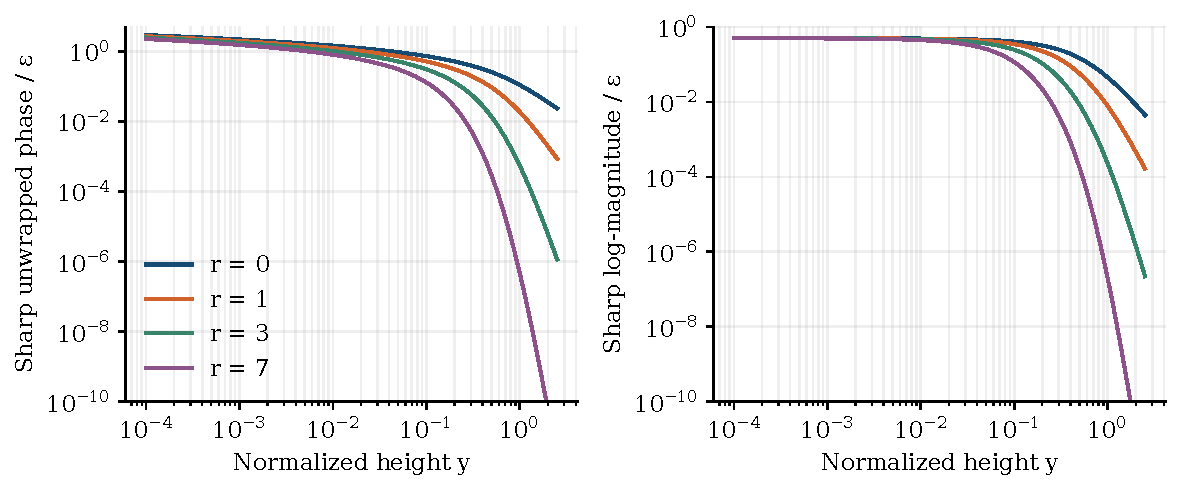
\includegraphics[width=\linewidth]{figures/budgets.pdf}
\caption{Exact marginal budgets for a unit log-error envelope.
Increasing calibration order reduces both at fixed height.
At fixed order, phase diverges logarithmically toward the band centre,
whereas log-magnitude tends to $1/2$.}
\label{fig:budgets}
\end{figure}

\begin{figure}[t]
\centering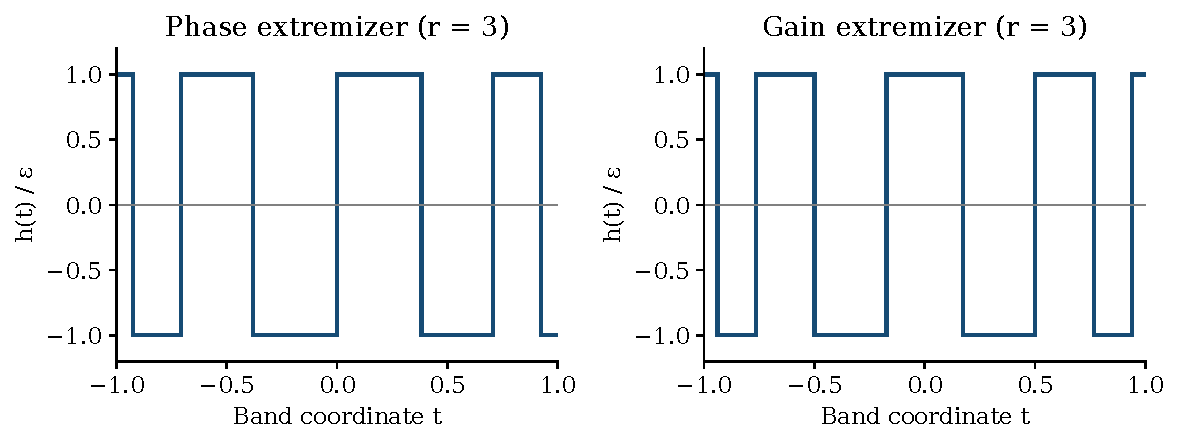
\includegraphics[width=\linewidth]{figures/extremizers.pdf}
\caption{Attaining perturbations with moments through degree six fixed.
The phase witness is odd and the gain witness even.
Their switches are second-kind Chebyshev roots.
The classical annihilating-sign identity supplies feasibility;
Theorem~\ref{thm:main} establishes their extremal factor error.}
\label{fig:witnesses}
\end{figure}

\subsection{Resolution and calibration order}
\begin{corollary}[Boundary resolution]\label{cor:resolution}
For fixed $r$ and $y\downarrow0$,
\[
 B_r(y)=\frac{\eps}{\pi}\log\frac{1}{(r+1)y}+o(1),
 \qquad A_r(y)\longrightarrow\frac{\eps}{2}.
\]
For fixed $y>0$ and $r\to\infty$, writing $a=\asinh y$,
\[
 B_r(y)\sim\frac{2\eps}{\pi}e^{-2(r+1)a},\qquad
 A_r(y)\sim\frac{2\eps}{\pi}e^{-(2r+3)a}.
\]
If $r\to\infty$, $y\downarrow0$, and $(r+1)y\to\lambda\in(0,\infty)$,
then $B_r(y)\to\eps\pi^{-1}\log\coth\lambda$.
\end{corollary}
\begin{proof}
Use $\asinh y\sim y$, $\coth s\sim1/s$ at zero,
$\log\coth s\sim2e^{-2s}$ at infinity, and $\arctan s\sim s$ at zero.
\end{proof}

For $\eps,\tau>0$, the least nonnegative integer order with $B_r(y)\leq\tau$ is
\begin{equation}\label{eq:order}
 r_{\min}=\max\left\{0,\
 \left\lceil\frac{\atanh(e^{-\pi\tau/\eps})}{\asinh y}\right\rceil-1\right\}.
\end{equation}
This is a rule for the specified polynomial-moment family, not a lower bound
for all calibration measurements. A measurement equal to the phase functional
could eliminate its uncertainty directly.
For example, with $\eps=0.02$ and target $\tau=0.001$, the rule requires
$r=127$ (255 moments) at $y=0.01$, but only $r=12$ (25 moments) at $y=0.1$.
Near an integer threshold, evaluate \eqref{eq:order} with interval arithmetic
rather than an unverified floating-point ceiling.

Parity explains which added moments help. Phase uses only odd $h$, so the
degree-$2r$ condition does not improve its budget beyond degree $2r-1$
for $r\geq1$. Gain uses only even $h$; degrees through $2r+1$ give the same
gain budget as degrees through $2r$.

\subsection{The joint set is smaller than its marginal rectangle}
The set
$\mathcal Z_m(z)=\{\C h(z):h\in\Hcal_m(\eps)\}$
is compact, centrally symmetric, and convex.
Weak-* compactness of the feasible set and integrability of the evaluation
kernels give compactness.
At $iy$, it lies in $[-A_r,A_r]+i[-B_r,B_r]$ when $m=2r$.
The unique gain maximizer is even, with zero centre phase;
the unique phase maximizer is odd, with zero centre gain.
Since both budgets are positive for $\eps>0$, no corner of that rectangle is
attainable. Two separately sharp bounds therefore do not give a jointly sharp
complex-error rectangle.
Figure~\ref{fig:joint} illustrates the geometry; directional continuum bounds
are developed in Section~\ref{sec:dual}.

\section{Inexact calibration and smooth perturbations}\label{sec:noisy}
\begin{theorem}[An inexact first moment]\label{thm:noisy}
Let $\norm h_\infty\leq\eps$ on $[-1,1]$ with $\eps>0$,
$\int h=\int t^2h=0$, and $|\int th|\leq\delta$.
Set $d=\min(\delta/\eps,1)$ and $a^2=(1+d)/2$.
The exact phase budget at $iy$ is
\begin{equation}\label{eq:noisy}
 B(y,\delta)=\frac{\eps}{2\pi}
 \log\frac{(y^2+a^2)^2}{y^2(1+y^2)}.
\end{equation}
For $0\leq\delta<\eps$ an attaining positive phase-integral witness is
$h(t)=\eps\sgn(t)\sgn(a^2-t^2)$.
For $\delta\geq\eps$ the constraint is inactive and $\eps\sgn t$ attains it.
\end{theorem}
\begin{proof}
The witness is odd, and its first moment is
$\eps(2a^2-1)=\min(\delta,\eps)$.
For $\delta<\eps$ choose $\lambda=(a^2+y^2)^{-1}$.
The residual
\[
 \frac{t}{t^2+y^2}-\lambda t
 =\frac{t(a^2-t^2)}{(t^2+y^2)(a^2+y^2)}
\]
has the witness's sign. Thus
\[
 \int\frac{th}{t^2+y^2}
 \leq\eps\int\left|\frac{t}{t^2+y^2}-\lambda t\right|+\lambda\delta,
\]
with equality for that witness. For $\delta\geq\eps$ use $\lambda=0$.
Integrating on $[0,a]$ and $[a,1]$ gives \eqref{eq:noisy}.
\end{proof}

At $\delta=0$ this is $B_1(y)$, while at $\delta=\eps$ it is $B_0(y)$.
The one-sided derivative at exact calibration is
\[
 \left.\frac{\partial B}{\partial\delta}\right|_{\delta=0}
 =\frac{1}{2\pi(y^2+1/2)}.
\]
The derivative stays finite as $y\downarrow0$: the first moment changes a
finite part of the budget but does not remove its boundary logarithm.

\begin{proposition}[Smooth perturbations have the same suprema]\label{prop:smooth}
For fixed finite $m$ and $\Imag z>0$, restricting $\Hcal_m(\eps)$ to real
$C^\infty$ functions compactly supported in $(-1,1)$ does not change the
supremum of any real linear combination of $\Real\C h(z)$ and $\Imag\C h(z)$.
\end{proposition}
\begin{proof}
Approximate a feasible $h$ by $h_\nu\in C_c^\infty(-1,1)$ with
$\norm{h_\nu}_\infty\leq\eps$ and $h_\nu\to h$ in $L^1$,
using cutoff and mollification. Its moment errors tend to zero.
Choose a nonnegative smooth bump $\eta$ supported in the interval and positive
on an open subinterval. For a basis $p_0,\ldots,p_m$, the matrix
$G_{jk}=\int\eta p_jp_k$ is positive definite.
Subtract $\eta\sum c_kp_k$ with $Gc=(\int p_jh_\nu)_j$.
This repairs the moments exactly; $c\to0$ and the correction's supremum
norm tends to zero.
For $\eps>0$, divide by
$1+\norm{\eta\sum c_kp_k}_\infty/\eps$.
The resulting functions are feasible, smooth, and converge to $h$ in $L^1$.
For fixed $\Imag z>0$, both evaluation kernels are bounded.
The case $\eps=0$ is immediate.
\end{proof}

This is smoothness without a fixed derivative bound.
A prescribed derivative or bandwidth restriction changes the uncertainty class
and may improve its budget.

\section{Weighted and off-centre budgets}\label{sec:dual}
For a direction $(u,v)\in\mathbb R^2$ define
\[
 k_{u,v,z}(t)=\frac{uy-v(t-x)}{(t-x)^2+y^2}.
\]
Then $u\Real\C h+v\Imag\C h=(2\pi)^{-1}\int k_{u,v,z}h$.
Let $b(t)>0$ almost everywhere be integrable, let $p_0,\ldots,p_m$ be a basis
of $\mathbb P_m$, and let $\delta_j\geq0$.
Consider real $h$ with $|h|\leq\eps b$ and $|\int p_jh|\leq\delta_j$.

\begin{theorem}[Directional best-$L^1$ formula]\label{thm:dual}
For $\eps>0$, $y>0$, and a nonzero direction, the exact support value is
\begin{equation}\label{eq:dual}
 \sup_h\frac{1}{2\pi}\int k_{u,v,z}h
 =\frac{1}{2\pi}\min_{\lambda\in\mathbb R^{m+1}}
 \left\{\eps\int_{-1}^{1}b(t)
 \left|k_{u,v,z}(t)-\sum_{j=0}^m\lambda_jp_j(t)\right|dt
 +\sum_{j=0}^m\delta_j|\lambda_j|\right\}.
\end{equation}
For exact moments the penalty vanishes; with $b=1$ this is ordinary best
$L^1$ polynomial approximation.
\end{theorem}
\begin{proof}
Subtract $p=\sum\lambda_jp_j$ inside the integral. The envelope and moment
bounds prove the right side is an upper bound for every $\lambda$.
On the polynomial space, $\int b|p|$ is a norm.
The objective is coercive and has a minimizer $\lambda_*$.
For a nonzero direction, $k-p_*$ is a nonzero rational function with only
finitely many zeros on the band. Differentiation of the integral term is
justified by domination.
Putting $s(t)=\sgn(k(t)-p_*(t))$, subgradient optimality gives
\[
 \eps\int b(t)s(t)p_j(t)\,dt
 \in \delta_j\partial|\lambda_{*,j}|.
\]
Hence $h_*=\eps b s$ satisfies the moment bounds and attains equality in
both the moment and pointwise absolute-value bounds.
\end{proof}

This is a specialization of established $L^1$ duality.
Its value here is computational: any candidate polynomial gives a continuum
upper bound when its absolute residual is correctly integrated.
With exact moments and $b=1$, the residual numerator has degree at most $m+2$,
so an optimal witness has at most $m+2$ interior switches.
Off centre, one canonical Chebyshev sign generally does not solve every
direction. Certified directional half-planes give an outer polygon for
$\mathcal Z_m(z)$, while feasible witnesses give an inner set.

\begin{figure}[t]
\centering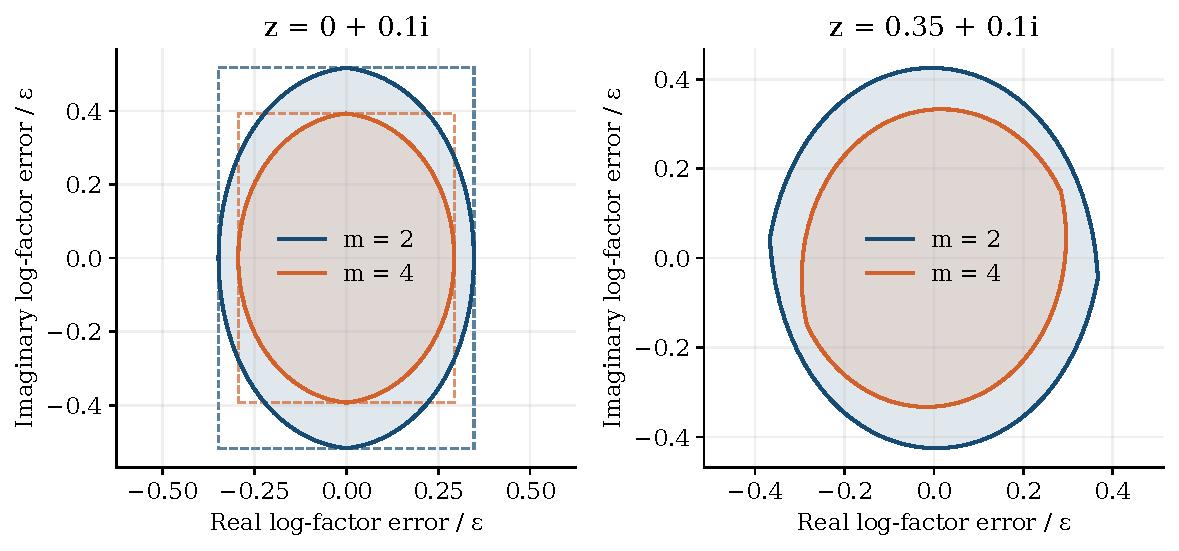
\includegraphics[width=\linewidth]{figures/joint_sets.pdf}
\caption{Joint uncertainty for two moment orders. Solid curves are
numerical LP candidate polygons with 512 cells and 97 sampled directions,
illustrating geometry rather than asserting exact continuum boundaries.
Dashed centre rectangles use the exact marginal budgets and have unattainable
corners. Separate continuum brackets appear in Table~\ref{tab:brackets}.}
\label{fig:joint}
\end{figure}

\section{Continuum certificates from finite searches}\label{sec:certificates}
The reference implementation, \texttt{PhaseBudgets}, separates optimization
from validation. The general certifier handles a constant envelope, exact
Legendre moments, rational $x,y$, and rational directions. It does not implement
every weighted or noisy case of Theorem~\ref{thm:dual}.

\subsection{Search and exact moment repair}
Partition the band into $N$ rational cells and take $h_0$ constant on each.
A linear program maximizes the functional with $-1\leq h_0\leq1$
and exactly integrated Legendre moment equations.
Kernel integrals on cells use logarithms and arctangents.
HiGHS, through SciPy, supplies cell values and dual multipliers.
These floating-point values are only proposals.

The certifier interprets every candidate decimal as an exact rational number,
clips heights to the declared box, and recomputes moments exactly.
For Legendre polynomials $P_j(1)=1$, set
\[
 \eta_j=\int_{-1}^{1}P_jh_0,\qquad
 q(t)=\sum_{j=0}^m\frac{2j+1}{2}\eta_jP_j(t),\qquad
 D=\sum_{j=0}^m\frac{2j+1}{2}|\eta_j|.
\]
Legendre orthogonality and $|P_j|\leq1$ imply that
\begin{equation}\label{eq:repair}
 \widehat h(t)=\frac{h_0(t)-q(t)}{1+D}
\end{equation}
has zero calibration moments and supremum norm at most one.
Its directional integral is a lower certificate.
Solver feasibility tolerances are therefore not mistaken for exact feasibility.

\subsection{Root-isolated integration}
The proposed dual is converted to a rational polynomial $p$.
The numerator of $k-p$ is
\[
 N(t)=uy-v(t-x)-((t-x)^2+y^2)p(t).
\]
SymPy isolates all its real band roots in rational intervals of width at most
$10^{-25}$. Between these boxes the sign is determined by an exact rational
sample, and the integral of $|k-p|$ is a signed antiderivative difference.
A root interval of width $\ell$ contributes at most
\[
 \ell\,\frac{\sum_j|N_j|}{y^2},\qquad N(t)=\sum_jN_jt^j.
\]
This follows from $|t|\leq1$ and the denominator bound $y^2$.

All logarithms, arctangents, and endpoint evaluations use Arb ball arithmetic
\cite{arb}. Integrals of polynomial multiples of $k$ use exact polynomial
division followed by polynomial, logarithmic, and arctangent terms.
Records retain rational root boxes and ball enclosures.
Exported floating-point endpoints are enlarged by one unit in the last place;
the recorded balls retain higher precision.

An inaccurate optimizer consequently leaves a wider bracket rather than
invalidating it. A finite cell grid is never used by itself as a continuum
upper bound. The interval result still depends on the correctness of its
algebraic and ball-arithmetic implementation.

\section{Computational study}\label{sec:experiments}
The deterministic synthetic experiments test the formulas, continuum
certification, and smooth near-attainment. They are not measurements of
deployed systems. Source, records, figure generation, dependency versions,
and automated checks accompany the manuscript.

\subsection{Closed forms and witnesses}
We use $r=0,\ldots,12$ and
$y\in\{0.001,0.01,0.1,0.3,1,3\}$.
Both formulas are compared with piecewise antiderivative evaluations at 192
and 384 bits, giving 312 comparisons.
The witnesses also give 4,056 ball checks of zero moments through degree
$2r$. Every difference or moment enclosure contains zero.
The proof of the identities is Theorem~\ref{thm:main};
these computations corroborate their implementation.

A separate mpmath implementation directly integrates each switch interval
for 12 phase cases:
$r\in\{0,1,3,6\}$, $y\in\{0.01,0.2,1\}$.
At 70 decimal digits, each absolute difference is below $10^{-60}$.
These are high-precision numerical comparisons rather than interval proofs.
An additional symbolic script verifies 14 polynomial-division identities exactly
and checks the canonical-sign transform at 15 off-axis points by separate
65-digit quadrature; the largest transform discrepancy is below $7.47\times10^{-64}$.

\begin{table}[t]
\centering\begin{tabular}{rrrrr}
\toprule
$r$ & Moments & $B_r(0.01)/\epsilon$ & $B_r(0.1)/\epsilon$ & $A_r(0.1)/\epsilon$\\
\midrule
0 & 1 & 1.465887 & 0.734519 & 0.406060\\
1 & 3 & 1.245283 & 0.517020 & 0.347324\\
3 & 7 & 1.024775 & 0.308511 & 0.246167\\
7 & 15 & 0.804648 & 0.130678 & 0.115349\\
12 & 25 & 0.651214 & 0.047577 & 0.042911\\
\bottomrule
\end{tabular}

\caption{Exact-law values rounded to six decimals.
The moment count includes every degree from zero through $2r$.
Phase and gain columns have different attaining perturbations.}
\label{tab:budgets}
\end{table}

At $y=0.01$, increasing the number of moments from one to 25 reduces the
normalized phase budget from $1.465887$ to $0.651214$.
At $y=0.1$ it decreases from $0.734519$ to $0.047577$.
These values illustrate the height-dependent transition, rather than uniform
removal of boundary sensitivity.

\subsection{Continuum brackets}
We test $m\in\{2,4\}$,
$(x,y)\in\{(0,0.1),(0.35,0.1),(0.35,0.5)\}$, and directions
$(1,0),(0,1),(1,1)$: 18 certificates with 256 cells.
Each repaired primal lower bound lies below its continuum dual upper bound.
The largest normalized gap is below $1.33\times10^{-4}$.
Table~\ref{tab:brackets} gives selected brackets with outward rounding.

\begin{table}[t]
\centering\begin{tabular}{rrrrrr}
\toprule
$m$ & $x$ & $y$ & Direction & Lower & Upper\\
\midrule
2 & 0 & 0.1 & $(0,1)$ & 0.517001 & 0.517020\\
2 & 0.35 & 0.1 & $(0,1)$ & 0.425340 & 0.425472\\
2 & 0.35 & 0.1 & $(1,1)$ & 0.547879 & 0.547967\\
2 & 0.35 & 0.5 & $(0,1)$ & 0.052280 & 0.052294\\
4 & 0 & 0.1 & $(0,1)$ & 0.393075 & 0.393125\\
4 & 0.35 & 0.1 & $(0,1)$ & 0.332960 & 0.333064\\
4 & 0.35 & 0.1 & $(1,1)$ & 0.462509 & 0.462586\\
4 & 0.35 & 0.5 & $(0,1)$ & 0.019082 & 0.019094\\
\bottomrule
\end{tabular}

\caption{Continuum support brackets for a unit envelope.
Direction $(u,v)$ means $u\Real\C h+v\Imag\C h$;
$(1,1)$ is not a unit direction.
Centre phase values agree with the closed laws.}
\label{tab:brackets}
\end{table}

A refinement study uses 32, 64, 128, 256, and 512 cells for phase at
$0+0.1i$ and $0.35+0.1i$, with $m=4$, adding ten certificates.
The recorded gaps decrease along these sequences.
Automated checks also replay four off-centre directions at 192 and 384 bits.
The general algorithm is a certificate-producing reference method; no
computational optimality or speedup over specialist $L^1$ solvers is claimed.

\subsection{Smoothness and calibration noise}
For a numerical realization of Proposition~\ref{prop:smooth}, use
\[
 \eta_\kappa(t)=
 \begin{cases}
 \exp[-1/(\kappa(1-t^2))],& |t|<1,\\
 0,& |t|\geq1,
 \end{cases}
 \qquad
 h_0(t)=\eta_\kappa(t)\tanh\!\big(\kappa(-1)^rU_{2r+1}(t)\big).
\]
Subtract $\eta_\kappa\sum c_jP_j$ using the bump-weighted Gram system,
then divide by $1+\sum|c_j|$.
This defines exactly feasible functions when its integrals are exact.
The experiment uses adaptive quadrature and a dense numerical solve;
it does not validate that Gram solve.

For $r\in\{1,3\}$, $\kappa\in\{8,32,128,512\}$, and
$y\in\{0.01,0.1\}$ there are 16 cases.
The largest numerically recomputed moment residual is below
$3.76\times10^{-16}$.
Figure~\ref{fig:robustness} shows increasing attainment of the sharp budget.
These results do not establish a law under a fixed derivative bound.

An independently assembled 4,096-cell LP checks
Theorem~\ref{thm:noisy} at $y=0.2$ for
$\delta/\eps\in\{0,0.1,0.5,1\}$.
Differences from the normalized formula are below $10^{-6}$.
The theorem establishes sharpness; the LP provides a numerical cross-check.

\begin{figure}[t]
\centering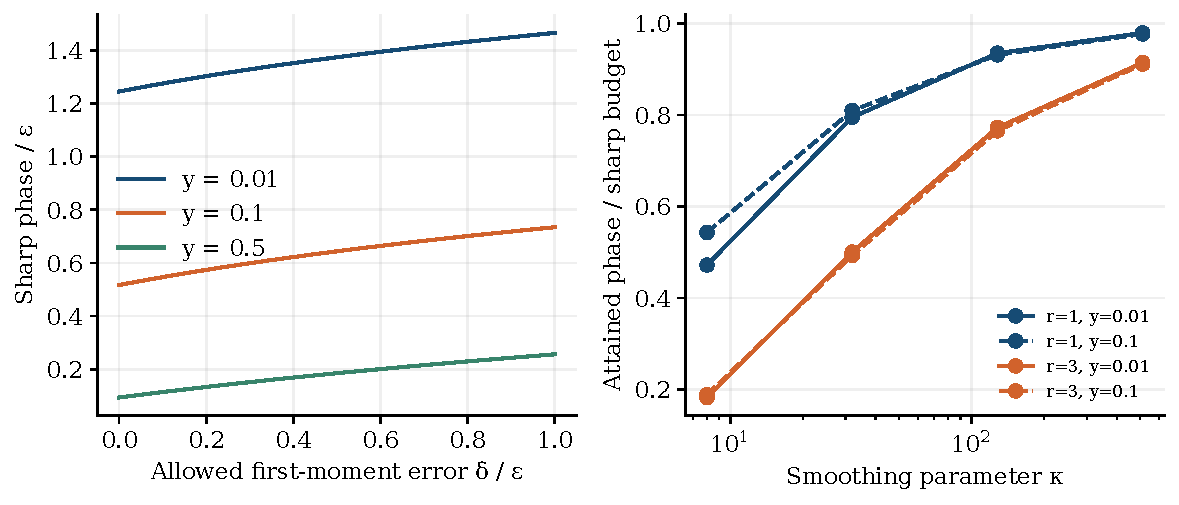
\includegraphics[width=\linewidth]{figures/robustness.pdf}
\caption{Left: the exact inexact-first-moment law, with mean and second
moment fixed. Right: numerical phase attainment after smooth moment repair
and norm rescaling. Smooth-case points use numerical quadrature;
Proposition~\ref{prop:smooth} supplies the continuum approximation statement.}
\label{fig:robustness}
\end{figure}

\subsection{A factor and inverse-factor example}
Take the positive reference symbol
\[
 K_0(t)=\frac{t^2+4}{t^2+1},\qquad K_{0,+}(z)=\frac{z+2i}{z+i}.
\]
The upper factor is analytic and zero-free in the upper half-plane and tends
to one at infinity.
For $K=K_0e^{h_B}$, the phase witness gives
\[
 \frac{K_+(iy)}{K_{0,+}(iy)}=e^{-iB_r(y)},\qquad
 e^{-\eps}\leq K/K_0\leq e^\eps.
\]
This is a factorization of an actual positive perturbed kernel, rather than
an unconstrained error imposed on its factor.
For the inverse factor $W_+=K_+^{-1}$, a building block of whitening and
Wiener--Hopf solution formulas, the ratio is $e^{iB_r(y)}$.

At $\eps=0.02$ and $y=0.01$, three moments give a sharp phase budget
of approximately $0.024906$ radians; 25 moments give $0.013024$ radians.
At $y=0.1$, the corresponding budgets are $0.010340$ and $0.000952$ radians.
For this phase-only witness the relative complex response difference is
$2|\sin(B_r/2)|$.
Over its scalar multiples, the largest circular discrepancy is
$2\sin(\min(B_r,\pi)/2)$, a distinction needed when unwrapped error exceeds $\pi$.

An interior complex evaluation is an exponentially regularized frequency
response, not an ordinary real-frequency measurement.
The example does not certify a closed-loop controller, a real-signal filter
with even spectral symmetry, or the solution of a complete physical problem.

\section{Use and limitations}
The immediate applications are selecting a calibration order or an interior
evaluation height under a justified log-error budget, and generating
adversarial positive symbols with known factor behavior.
An engineering integration must obtain the band support, envelope, and moment
tolerances from its own acquisition or approximation procedure.

The model assumes exact information outside the band. Uncertain external tails
require additional envelopes and integrals. The centre laws use a constant
envelope and unweighted polynomial moments. Matrix factorization does not
generally reduce to commuting scalar logarithms. Even-spectrum constraints
remove the centre-phase problem. Smoothness without a derivative budget
preserves the supremum; a fixed regularity bound may not.

The off-centre implementation is tested at low moment orders.
Exact algebra and root isolation may become expensive at larger orders.
The certifier checks proposed functions rather than proving a third-party
optimizer correct. This makes optimizer accuracy dispensable for soundness,
but retains the explicit dependency on the algebraic and interval libraries.

Further work could optimize over experimentally available calibration
functionals, rather than increasing a fixed polynomial family.
Adding a derivative budget would replace the free sign extremizers by a
different constrained control problem. Neither extension is resolved here.

\section{Conclusion}
Positive scalar kernels with bounded finite-band logarithmic uncertainty
admit exact marginal factor-error laws under polynomial calibration.
Chebyshev sign functions attain both laws, separately, and smooth compactly
supported perturbations approach the same suprema.
The phase budget separates exponential improvement at fixed complex height
from the boundary sensitivity retained by every fixed moment order.
Best-$L^1$ duality and checked primal--dual brackets extend the calculation
beyond the closed-form centre case, providing an auditable accuracy interface
for scalar Wiener--Hopf factorization.

\section*{Data and software availability}
The artifact is available at \url{https://github.com/shi1720/phasebudgets}.
Commands \texttt{python run\_experiments.py},
\texttt{python make\_figures.py}, and
\texttt{python -m unittest discover -s tests -v}
regenerate records, figures, tables, and tests.
The saved environment uses Python 3.12.14, NumPy 2.5.4,
SciPy 1.18.1, mpmath 1.3.0, and python-flint 0.9.0.
The manifest records actual versions.
Figures are generated from the formulas and saved measurements.

\begin{thebibliography}{10}
\bibitem{review}
A. V. Kisil, I. D. Abrahams, G. Mishuris, and S. V. Rogosin,
The Wiener--Hopf technique, its generalizations and applications:
constructive and approximate methods,
\emph{Proc. R. Soc. A} 477 (2021), 20210533.
\href{https://doi.org/10.1098/rspa.2021.0533}{doi:10.1098/rspa.2021.0533}.

\bibitem{kisil}
A. V. Kisil,
A constructive method for an approximate solution to scalar Wiener--Hopf equations,
\emph{Proc. R. Soc. A} 469 (2013), 20120721.
\href{https://doi.org/10.1098/rspa.2012.0721}{doi:10.1098/rspa.2012.0721}.

\bibitem{anderson}
B. D. O. Anderson and M. Green,
Hilbert transform and gain/phase error bounds for rational functions,
\emph{IEEE Trans. Circuits Syst.} 35 (1988), 528--535.
\href{https://doi.org/10.1109/31.1780}{doi:10.1109/31.1780}.

\bibitem{sandberg}
H. Sandberg, A. Lanzon, and B. D. O. Anderson,
Transfer function approximation and identification using magnitude and phase criteria,
in \emph{Proc. 17th International Symposium on Mathematical Theory of Networks
and Systems}, Kyoto, 2006, pp. 250--256.
\href{https://mathweb.ucsd.edu/~helton/MTNSHISTORY/CONTENTS/2006KYOTO/CONFERENCEWEBSITE/papers/0115.pdf}{Conference paper}.

\bibitem{boche}
H. Boche and V. Pohl,
Behaviour of the spectral factorization for continuous spectral densities,
\emph{Signal Processing} 87 (2007), 1078--1088.
\href{https://doi.org/10.1016/j.sigpro.2006.10.002}{doi:10.1016/j.sigpro.2006.10.002}.

\bibitem{ephremidze}
L. Ephremidze, E. Shargorodsky, and I. Spitkovsky,
Quantitative results on continuity of the spectral factorization mapping in the
scalar case, \emph{Bol. Soc. Mat. Mex.} 22 (2016), 517--527.
\href{https://doi.org/10.1007/s40590-016-0117-7}{doi:10.1007/s40590-016-0117-7}.

\bibitem{palmer}
K. F. Palmer, M. Z. Williams, and B. A. Budde,
Multiply subtractive Kramers--Kronig analysis of optical data,
\emph{Applied Optics} 37 (1998), 2660--2673.
\href{https://doi.org/10.1364/AO.37.002660}{doi:10.1364/AO.37.002660}.

\bibitem{hobby}
C. R. Hobby and J. R. Rice,
A moment problem in $L_1$ approximation,
\emph{Proc. Amer. Math. Soc.} 16 (1965), 665--670.

\bibitem{nakatsukasa}
Y. Nakatsukasa and A. Townsend,
Error localization of best $L_1$ polynomial approximants,
\emph{SIAM J. Numer. Anal.} 59 (2021), 314--333.
\href{https://doi.org/10.1137/19M1242860}{doi:10.1137/19M1242860}.

\bibitem{arb}
F. Johansson,
Arb: efficient arbitrary-precision midpoint-radius interval arithmetic,
\emph{IEEE Trans. Computers} 66 (2017), 1281--1292.
\href{https://doi.org/10.1109/TC.2017.2690633}{doi:10.1109/TC.2017.2690633}.
\end{thebibliography}
\end{document}
